\section{Fundamentos teóricos}

\subsection{Referencias}
Este es un texto de muestra como ejemplo.

Las referencias deben ser completas con formato bibtex en el archivo 'ref.bib'.
Puede luego citar las referencias como \cite{ex}.

\subsection{Circuitos en Latex}

Los circuitos pueden ser editados empleando Latex~.

\begin{center}
\begin{circuitikz} \draw
(0,0) to[bandpass, l^=$RF$] (1.5,0)
(1.5,0) to[amp] (3,0)

(3.5,0) node[mixer]{}
(4,-2) node[oscillator]{}
(3.5,-1.5) to[short] (3.5,-0.5)

(4,0) to[bandpass, l^=$1IF$] (5.5,0)
(5.5,0) to[amp] (7,0)

(7.5,0) node[mixer]{}
(8,-2) node[oscillator]{}
(7.5,-1.5) to[short] (7.5,-0.5)

(8,0) to[bandpass, l^=$2IF$] (9.5,0)
(9.5,0) to[vamp] (12.5,0)

(11,-2) to[short] (11,-0.4)
(12.5,-2) to[twoport,l=$AGC$] (11,-2)
(12.5,-2) to[short] (12.5,0);

\end{circuitikz}

\end{center}


\subsection{Imágenes}
Las imágenes pueden ser incluidas como se muestra a continuación.

\subsubsection{Una columna}
\begin{figure}[ht]
	\centering
	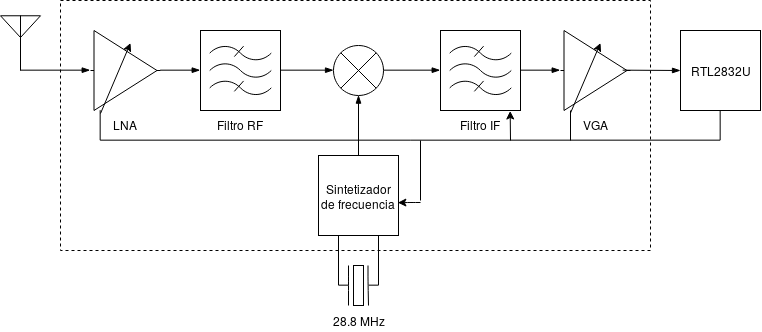
\includegraphics[width=0.8\linewidth]{fig/frontend.png}
	\caption{Esto es un diagrama.}
	\label{fig:diagrama}
\end{figure}


\subsubsection{Dos columnas}
Las imágenes pueden ser también puestas en dos columnas, como se muestra en el ejemplo siguiente.

\begin{figure}[ht]
	\centering
	\begin{minipage}[c]{0.4\linewidth}
		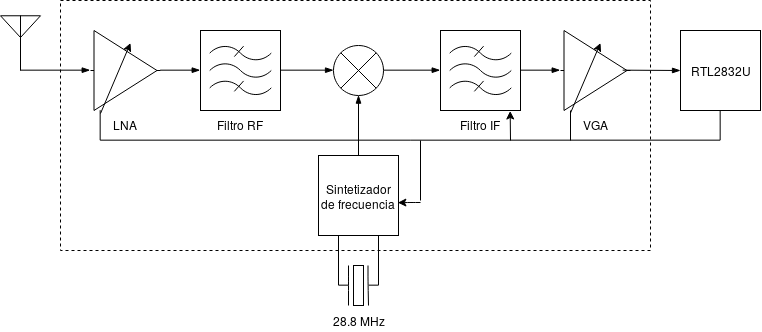
\includegraphics[width=0.9\linewidth]{fig/frontend.png}
		\caption{Esto es un diagrama.}
		\label{fig:logo1}
	\end{minipage}
	\hspace{0.4cm}
	\begin{minipage}[c]{0.4\linewidth}
		
\includegraphics[width=0.9\linewidth]{fig/UTNFRBA.png}
		\caption{Darker logo}
		\label{fig:logo2}
	\end{minipage}%
\end{figure}



